\documentclass[12pt,a4paper]{article}
\usepackage[french]{babel}
\usepackage[T1]{fontenc}
\usepackage{lmodern}
\usepackage[utf8]{inputenc}
\usepackage{amsmath}
\usepackage{amsfonts}
\usepackage{amssymb}
\usepackage{graphicx}
\usepackage{hyperref}
\usepackage{titlesec}
\usepackage{geometry}
\usepackage{tikz} % Pour les cadres et effets
\usepackage{xcolor} % Pour les couleurs


\usepackage{geometry}
\geometry{margin=2.5cm}
\usepackage{graphicx}
\usepackage{hyperref}
\usepackage{fancyhdr}
\pagestyle{fancy}
\fancyhf{}
\rhead{Gradient Conjugué}
\lhead{Matrices Creuses}
\cfoot{\thepage}

%-----
\usepackage{amsmath}  % Pour les formules mathématiques
\usepackage{booktabs} % Pour de beaux tableaux
\usepackage{array} 

\usepackage{amsmath,amsfonts}
\usepackage{geometry}
\usepackage{graphicx}
\geometry{margin=2.5cm}

\usepackage{graphicx}   % Pour insérer des images
\usepackage{listings}   % Pour afficher du code
\usepackage{xcolor}     % Pour la coloration syntaxique
\usepackage{caption}    % Pour les légendes personnalisées
\usepackage{float}      % Pour le placement des figures
\usepackage[utf8]{inputenc}  % Important pour les accents
\usepackage[T1]{fontenc}     % Améliore le rendu des caractères accentués

\lstset{
	% ... (votre configuration existante) ...
	literate=              % Gestion des accents
	{é}{{\'e}}1
	{è}{{\`e}}1
	{ê}{{\^e}}1
	{ë}{{\"e}}1
	{û}{{\^u}}1
	{ù}{{\`u}}1
	{â}{{\^a}}1
	{à}{{\`a}}1
	{î}{{\^i}}1
	{ô}{{\^o}}1
	{ç}{{\c c}}1
	{É}{{\'E}}1
	{È}{{\`E}}1
	{Ê}{{\^E}}1
	{À}{{\`A}}1
	{Â}{{\^A}}1
	{Î}{{\^I}}1
	{Ô}{{\^O}}1
	{Ç}{{\c C}}1
}

\lstset{
	language=Java,
	basicstyle=\ttfamily\small,
	keywordstyle=\color{blue},
	commentstyle=\color{gray},
	stringstyle=\color{red},
	breaklines=true,
	frame=single,
	showstringspaces=false,
	numbers=left,
	numberstyle=\tiny\color{gray},
	inputencoding=utf8,
	extendedchars=true,
	literate={é}{{\'e}}1 {è}{{\`e}}1 {à}{{\`a}}1 {ù}{{\`u}}1 {ç}{{\c{c}}}1
}

%%%%%%%%%%%%%%%%%%%%%%%%%%%%%%%%%

\geometry{hmargin=2.5cm,vmargin=2.5cm}

% Définition de la couleur bleu-gris
\definecolor{bluegray}{RGB}{200,220,240}

\begin{document}
	
	% Page de garde
	\begin{titlepage}
		\centering
		
		% Logo de l'institut
		\textsc{\LARGE Institut National Supérieur\\[0.5cm] d'Informatique}\\[1.5cm]
		
		
\includegraphics[width=0.3\textwidth]{logo.jpg}\\[1cm]
		
		% Cadre avec bords arrondis et fond bleu-gris
		
		
		%%%%%%%%%%%%%%%%%%%%%
		\begin{center}
			\begin{tikzpicture}
				\node[rectangle,
				rounded corners=15pt,
				inner sep=15pt,
				fill=bluegray,
				draw=blue!50!black,
				line width=1.5pt,
				text width=0.9\linewidth,  % Réduire légèrement la largeur
				align=center] (box) {      % Ajout crucial: align=center
					\fontsize{20}{24}\selectfont\bfseries
					Mini-projet 6 : Méthode du Gradient Conjugué pour Matrices Creuses
					
				};
			\end{tikzpicture}
		\end{center}
		%%%%%%%%%
        \vfill
		
		\begin{flushleft}
			\large
			\textbf{Spécialité :} I2AD\\
			\textbf{Niveau :} Master 1 \\
			\textbf{Semestre :} 7 \\
			\textbf{UE :} Algèbre linéaire  \\
			\textbf{Enseignant :} Dr. Dimby \\
			\textbf{Étudiante :} ANDRIATSIFERANA No Kanto Lorida\\
            \textbf{Étudiant :} ZO Manampisoa Hermann\\
			\textbf{Année académique :} 2025 - 2026
		\end{flushleft}
		
		\vspace{1cm}
		
		\begin{center}
			\today
		\end{center}
	\end{titlepage}
	
	\newpage
	\section*{Résumé }
	Ce mini-projet porte sur l'implémentation et l'étude de la méthode du gradient conjugué pour la résolution de systèmes linéaires dont la matrice est creuse, symétrique et définie positive. Le projet s'appuie sur des fondements mathématiques solides et se décline en plusieurs volets : génération de matrices creuses types (notamment la matrice de Poisson 2D), résolution par gradient conjugué avec et sans préconditionneur, analyse de la convergence, et comparaison entre les bibliothèques \texttt{NumPy} et \texttt{SciPy}.
	
	\section{Concepts mathématiques}
	
	\subsection{Définition du problème}
	Nous cherchons à résoudre un système linéaire de la forme :
	\begin{equation}
		Ax = b
	\end{equation}
	où $A \in \mathbb{R}^{n \times n}$ est une matrice symétrique définie positive et creuse, $x$ le vecteur inconnu, et $b$ un vecteur donné.

    	\subsection{ Génération de la matrice creuse (Poisson 2D)}
	
	\textbf{Contexte :} Le Laplacien 2D est un opérateur différentiel discret utilisé pour modéliser des phénomènes physiques comme la diffusion ou la chaleur.
	
	\textbf{Discrétisation :} On discrétise le domaine 2D (par exemple, un carré unité) avec une grille régulière. Cela transforme l’équation :
	\[
	- \Delta u(x, y) = f(x, y)
	\]
	en un système linéaire :
	\[
	A u = f
	\]
	où $A$ est une matrice creuse symétrique définie positive de taille $n^2 \times n^2$.
	
	\subsection{ Méthode du Gradient Conjugué (CG)}
	
	\textbf{Problème :} Résoudre $Ax = b$ quand $A$ est symétrique définie positive.
	\\ 
	\textbf{Principe :} C’est une méthode itérative qui construit une suite de vecteurs $x_0, x_1, x_2, \dots$ convergeant vers la solution.
	\newpage
	\subsubsection*{Algorithme du Gradient Conjugué}
	
	\begin{enumerate}
		\item Initialisation :
		\[
		x_0 = 0,\quad r_0 = b - Ax_0,\quad p_0 = r_0
		\]
		
		\item Pour $k = 0, 1, 2, \dots$ :
		\[
		\alpha_k = \frac{r_k^T r_k}{p_k^T A p_k}
		\]
		\[
		x_{k+1} = x_k + \alpha_k p_k
		\]
		\[
		r_{k+1} = r_k - \alpha_k A p_k
		\]
		Si $\|r_{k+1}\|$ est petit, on arrête.
		\[
		\beta_k = \frac{r_{k+1}^T r_{k+1}}{r_k^T r_k}
		\]
		\[
		p_{k+1} = r_{k+1} + \beta_k p_k
		\]
	\end{enumerate}
	
	\textbf{Remarque :} À chaque itération, la nouvelle direction $p_k$ est choisie de manière à être conjuguée aux précédentes. Cela permet d’accélérer la convergence.
	
	\subsection{ Visualisation de la convergence}
	
	\textbf{Erreur :} On peut visualiser :
	
	\begin{itemize}
		\item L’erreur absolue $\|x_k - x^*\|$ si la solution exacte $x^*$ est connue.
		\item Le résidu $\|r_k\|$ si $x^*$ est inconnu.
	\end{itemize}
	
	\textbf{Graphe :} On peut tracer la courbe $\log(\|r_k\|)$ en fonction du nombre d’itérations pour observer la vitesse de convergence.
	
	\subsection{ Préconditionneurs}
	
	\textbf{Objectif :} Accélérer la convergence du gradient conjugué en transformant le système.
	
	On résout :
	\[
	M^{-1} A x = M^{-1} b
	\]
	au lieu de $Ax = b$, où $M$ est un approximant de $A$ plus simple à inverser.
	
	\subsubsection*{Exemples classiques}
	
	\begin{itemize}
		\item \textbf{Préconditionneur de Jacobi :}
		$
		M = diag(A)
		$
		On divise chaque composante du résidu par la diagonale de $A$.
		\item \textbf{Préconditionneur SSOR (Symmetric Successive Over-Relaxation) :} 
		Ce préconditionneur repose sur la décomposition $A = D + L + L^T$, avec $D$ la diagonale, $L$ la partie triangulaire inférieure. Il est plus efficace que Jacobi mais plus coûteux.
	\end{itemize}
	
    \newpage
	\section{Méthodologie}

    \subsection{Génération de la matrice de Poisson 2D}
    Le problème considéré est la résolution de l'équation de Poisson :
    \[
    -\Delta u(x, y) = f(x, y), \quad (x, y) \in \Omega = [0,1]^2
    \]
    avec conditions de Dirichlet homogènes. La discrétisation par différences finies sur une grille régulière de taille $n \times n$ donne un système linéaire $Ax = b$, où $A$ est une matrice creuse de taille $n^2 \times n^2$, symétrique définie positive.

    \subsection{Méthode du Gradient Conjugué}
    Le gradient conjugué (CG) est utilisé pour résoudre $Ax = b$, avec les variantes suivantes :

    \begin{itemize}
        \item \textbf{Sans préconditionneur} : CG classique.
        \item \textbf{Avec préconditionneur Jacobi} : $M = \text{diag}(A)$.
        \item \textbf{Avec préconditionneur SSOR} : basé sur la décomposition $A = D + L + L^T$.
    \end{itemize}

    Le critère d'arrêt est basé sur la norme du résidu $\|r_k\| < 10^{-8}$. Les performances sont mesurées en nombre d’itérations et temps d’exécution.

    \subsection{Implémentations NumPy et SciPy}
    Deux implémentations ont été comparées :
    \begin{itemize}
        \item \textbf{Implémentation NumPy} : code manuel basé sur l’algorithme CG.
        \item \textbf{Fonction SciPy} : \texttt{scipy.sparse.linalg.cg} avec support natif pour les préconditionneurs via l’option \texttt{M=}.
    \end{itemize}
    \newpage
    \section{Résultats et Analyse}

    \subsection{Convergence : Implémentation NumPy}
    \begin{figure}[h!]
        \centering
        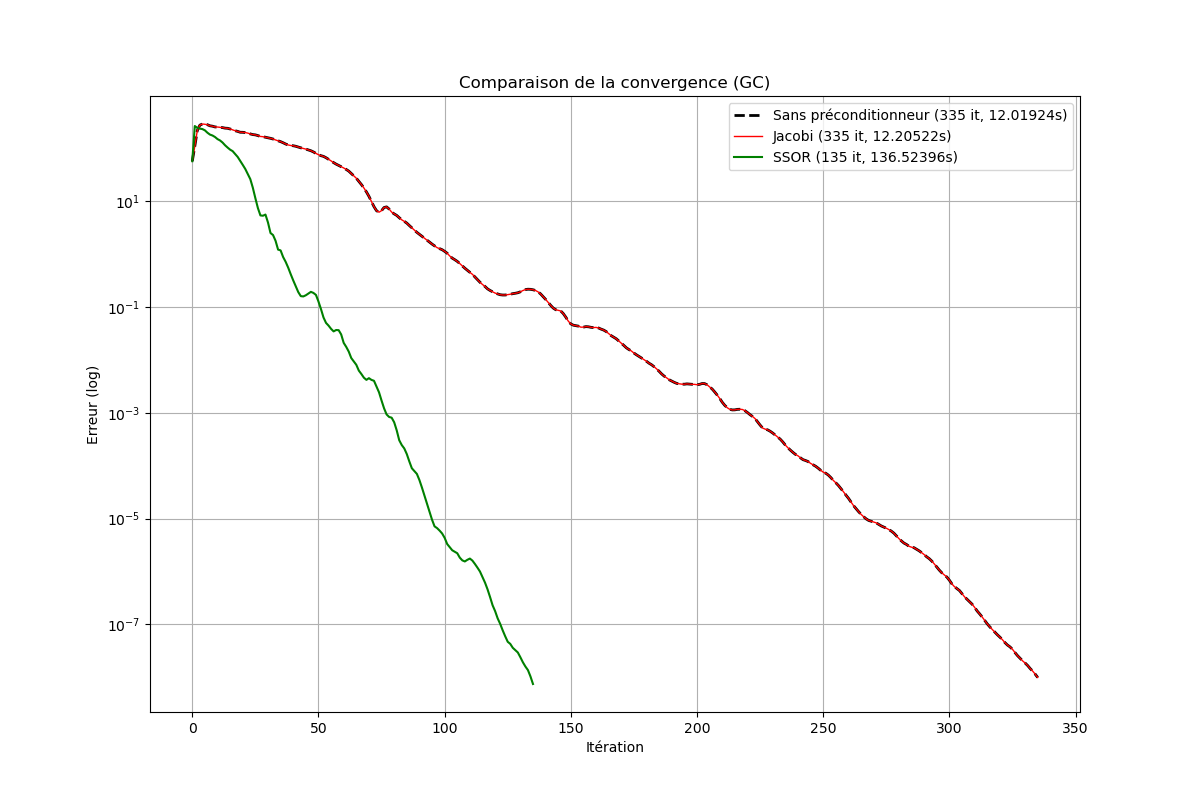
\includegraphics[width=\textwidth]{Comparaison_de_la_convergence_numpy.png}
        \caption{Convergence (implémentation NumPy) : CG sans préconditionneur, Jacobi, et SSOR}
        \label{fig:convergence_numpy}
    \end{figure}

    Les résultats montrent que :
    \begin{itemize}
        \item Sans préconditionneur et avec Jacobi, le nombre d’itérations est identique ($335$), avec un léger avantage en temps pour la version sans préconditionneur.
        \item Le préconditionneur SSOR réduit drastiquement les itérations ($135$) mais son coût de calcul élevé (\texttt{136 s}) le rend peu optimal dans ce contexte.
    \end{itemize}
    \vspace{1cm}
    \newpage
    \subsection{Convergence : Fonction SciPy}
    \begin{figure}[h!]
        \centering
        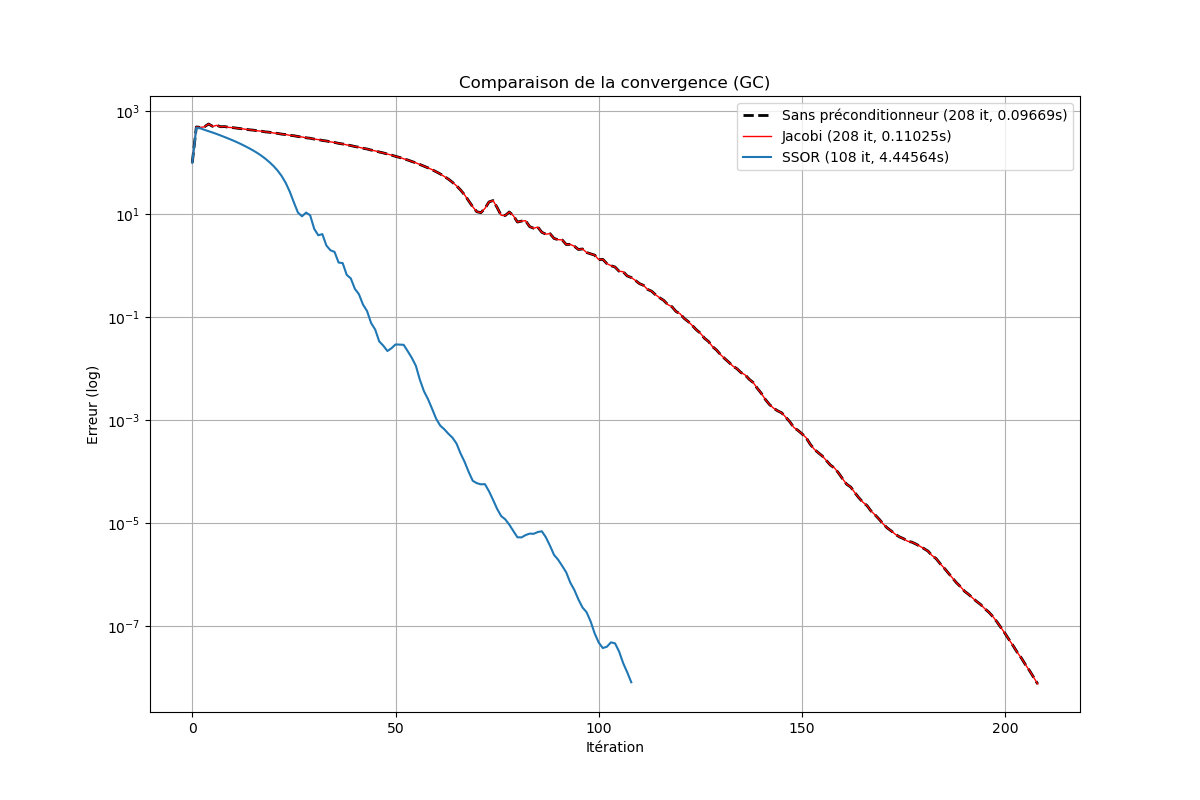
\includegraphics[width=\textwidth]{Comparaison_de_la_convergence_scipy.png}
        \caption{Convergence (fonction SciPy) : CG sans préconditionneur, Jacobi, et SSOR}
        \label{fig:convergence_scipy}
    \end{figure}

    Les observations sont similaires à celles obtenues avec NumPy. SciPy donne :
    \begin{itemize}
        \item Même nombre d'itérations pour Jacobi et sans préconditionneur ($208$), avec un léger gain de temps pour la version sans préconditionneur.
        \item Le préconditionneur SSOR divise presque par deux le nombre d’itérations ($108$) mais reste plus coûteux en temps d'exécution.
    \end{itemize}



    \newpage
    \section{Comparaison des approches NumPy et SciPy}
	
	La table suivante résume les différences essentielles entre les deux approches du projet :
	
	\begin{center}
		\begin{tabular}{|l|c|c|}
			\hline
			\textbf{Critère} & \textbf{NumPy (manuel)} & \textbf{SciPy (optimisé)} \\
			\hline
			Langage utilisé & Python + NumPy & Python + SciPy \\
			\hline
			Fonction CG & Codée à la main & \texttt{scipy.sparse.linalg.cg} \\
			\hline
			Préconditionneur Jacobi & Implémenté manuellement & Utilisé via \texttt{LinearOperator} \\
			\hline
			Préconditionneur SSOR & Implémenté manuellement & Utilisé via \texttt{LinearOperator} \\
			\hline
			Nombre d'itérations (Jacobi) & 335 & 208 \\
			\hline
			Nombre d'itérations (SSOR) & 135 & 108 \\
			\hline
			Facilité d’utilisation & Moins pratique & Très pratique \\
			\hline
			Contrôle de l’algorithme & Total & Limité \\
			\hline
			Performance & Bonne mais lente (SSOR) & Optimisée (multithreadée) \\
			\hline
		\end{tabular}
	\end{center}
	
	\textbf{Analyse} : SciPy offre un environnement plus rapide et pratique pour les grands systèmes linéaires creux. Cependant, l’implémentation manuelle en NumPy permet de comprendre en profondeur le fonctionnement de l’algorithme, ce qui est essentiel en contexte pédagogique.
	
	\section{Conclusion}
	
	Les tests effectués montrent que le choix du préconditionneur a un impact majeur sur la convergence du gradient conjugué :
	\begin{itemize}
		\item Le préconditionneur Jacobi est simple à implémenter mais n’améliore pas le nombre d’itérations.
		\item SSOR accélère la convergence en termes d’itérations, mais au prix d’un temps de calcul très élevé.
		\item SciPy permet une implémentation rapide et fiable, mais reste sensible au même compromis entre précision et performance.
	\end{itemize}
	
	L’algorithme du gradient conjugué reste donc très dépendant du préconditionneur et du contexte d’utilisation (temps réel ou précision extrême).


\end{document}
